% =========================================================
\section{The Abstraction: Address Spaces}
% =========================================================

\begin{frame}{Early Systems}
    \begin{columns}
        \begin{column}{0.55\textwidth}
            \begin{itemize}
                \item Early machines provided little memory abstraction.
                \item The OS occupied a fixed region of physical memory.
                \item A single running program used the remaining memory.
                \item There were few ``illusions'' provided by the OS.
            \end{itemize}
        \end{column}

        \begin{column}{0.42\textwidth}

        \begin{figure}
            \centering
            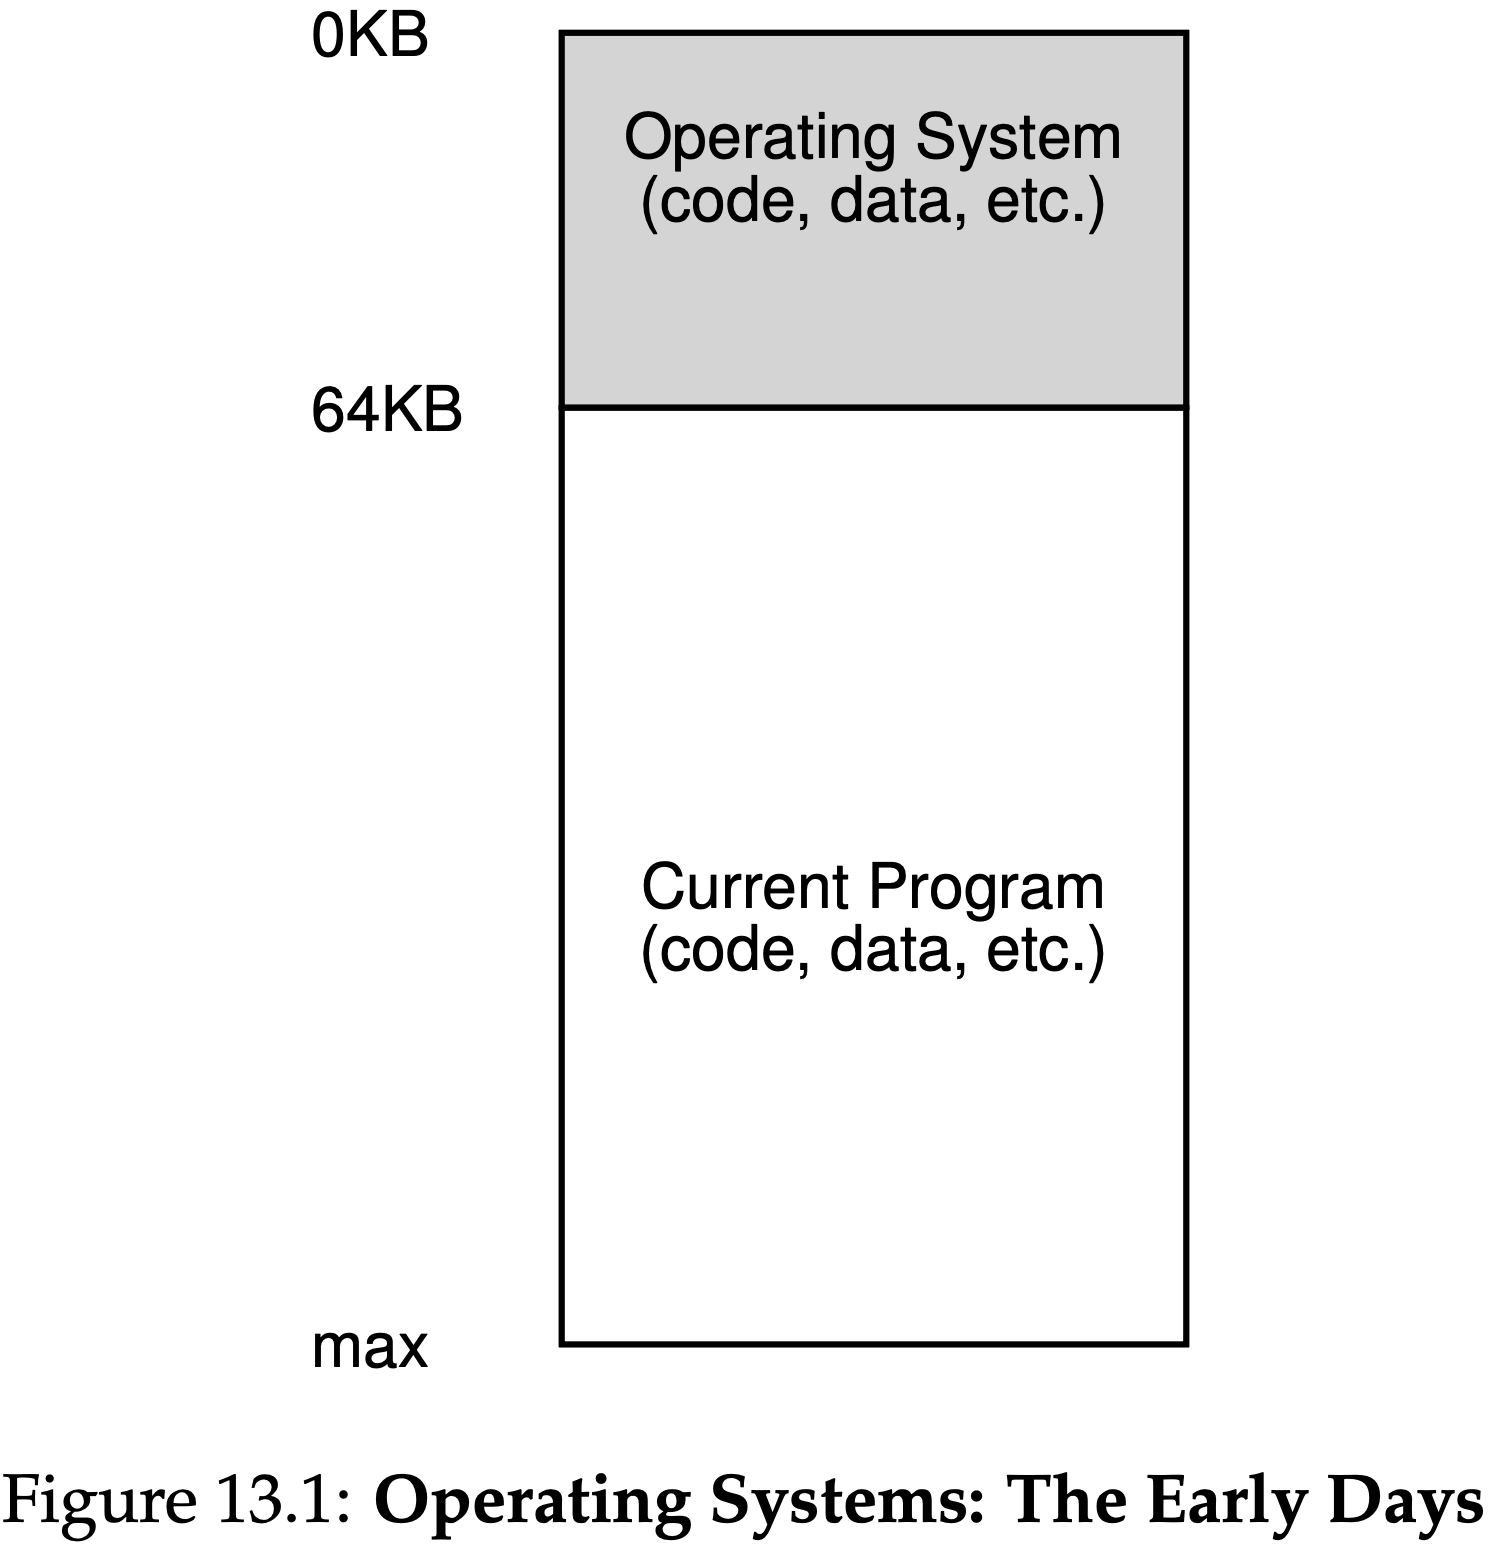
\includegraphics[width=1.1\linewidth]{figs/chapter-13/figure-13.1.png}
            \caption*{Source: chapter page 2.}
            \label{fig:figure-13.1}
        \end{figure}

        \end{column}
    \end{columns}
\end{frame}


\begin{frame}{Multiprogramming and Time Sharing}
    \begin{itemize}
        \item \textbf{Multiprogramming}: multiple processes are ready
              to run; the OS switches among them, e.g., during I/O.
        \item Main goal: improve CPU utilization.
        \pause
        \item \textbf{Time sharing}: multiple users interact with the
              machine and expect timely responses.
        \item Saving/restoring the entire memory to disk at each switch
              would be prohibitively slow.
        \item Better approach: keep multiple processes in memory and
              switch the CPU among them.
    \end{itemize}
\end{frame}


\begin{frame}{Sharing Physical Memory}
    \begin{columns}
        \begin{column}{0.50\textwidth}
            \begin{itemize}
                \item Multiple processes reside simultaneously in
                      physical memory.
                \item With one CPU, only one process runs at a time;
                      the others wait in the ready queue.
                \item This makes \textbf{protection} essential:
                      one process must not read or modify another
                      process's memory.
            \end{itemize}
        \end{column}

        \begin{column}{0.47\textwidth}

        \begin{figure}
            \centering
            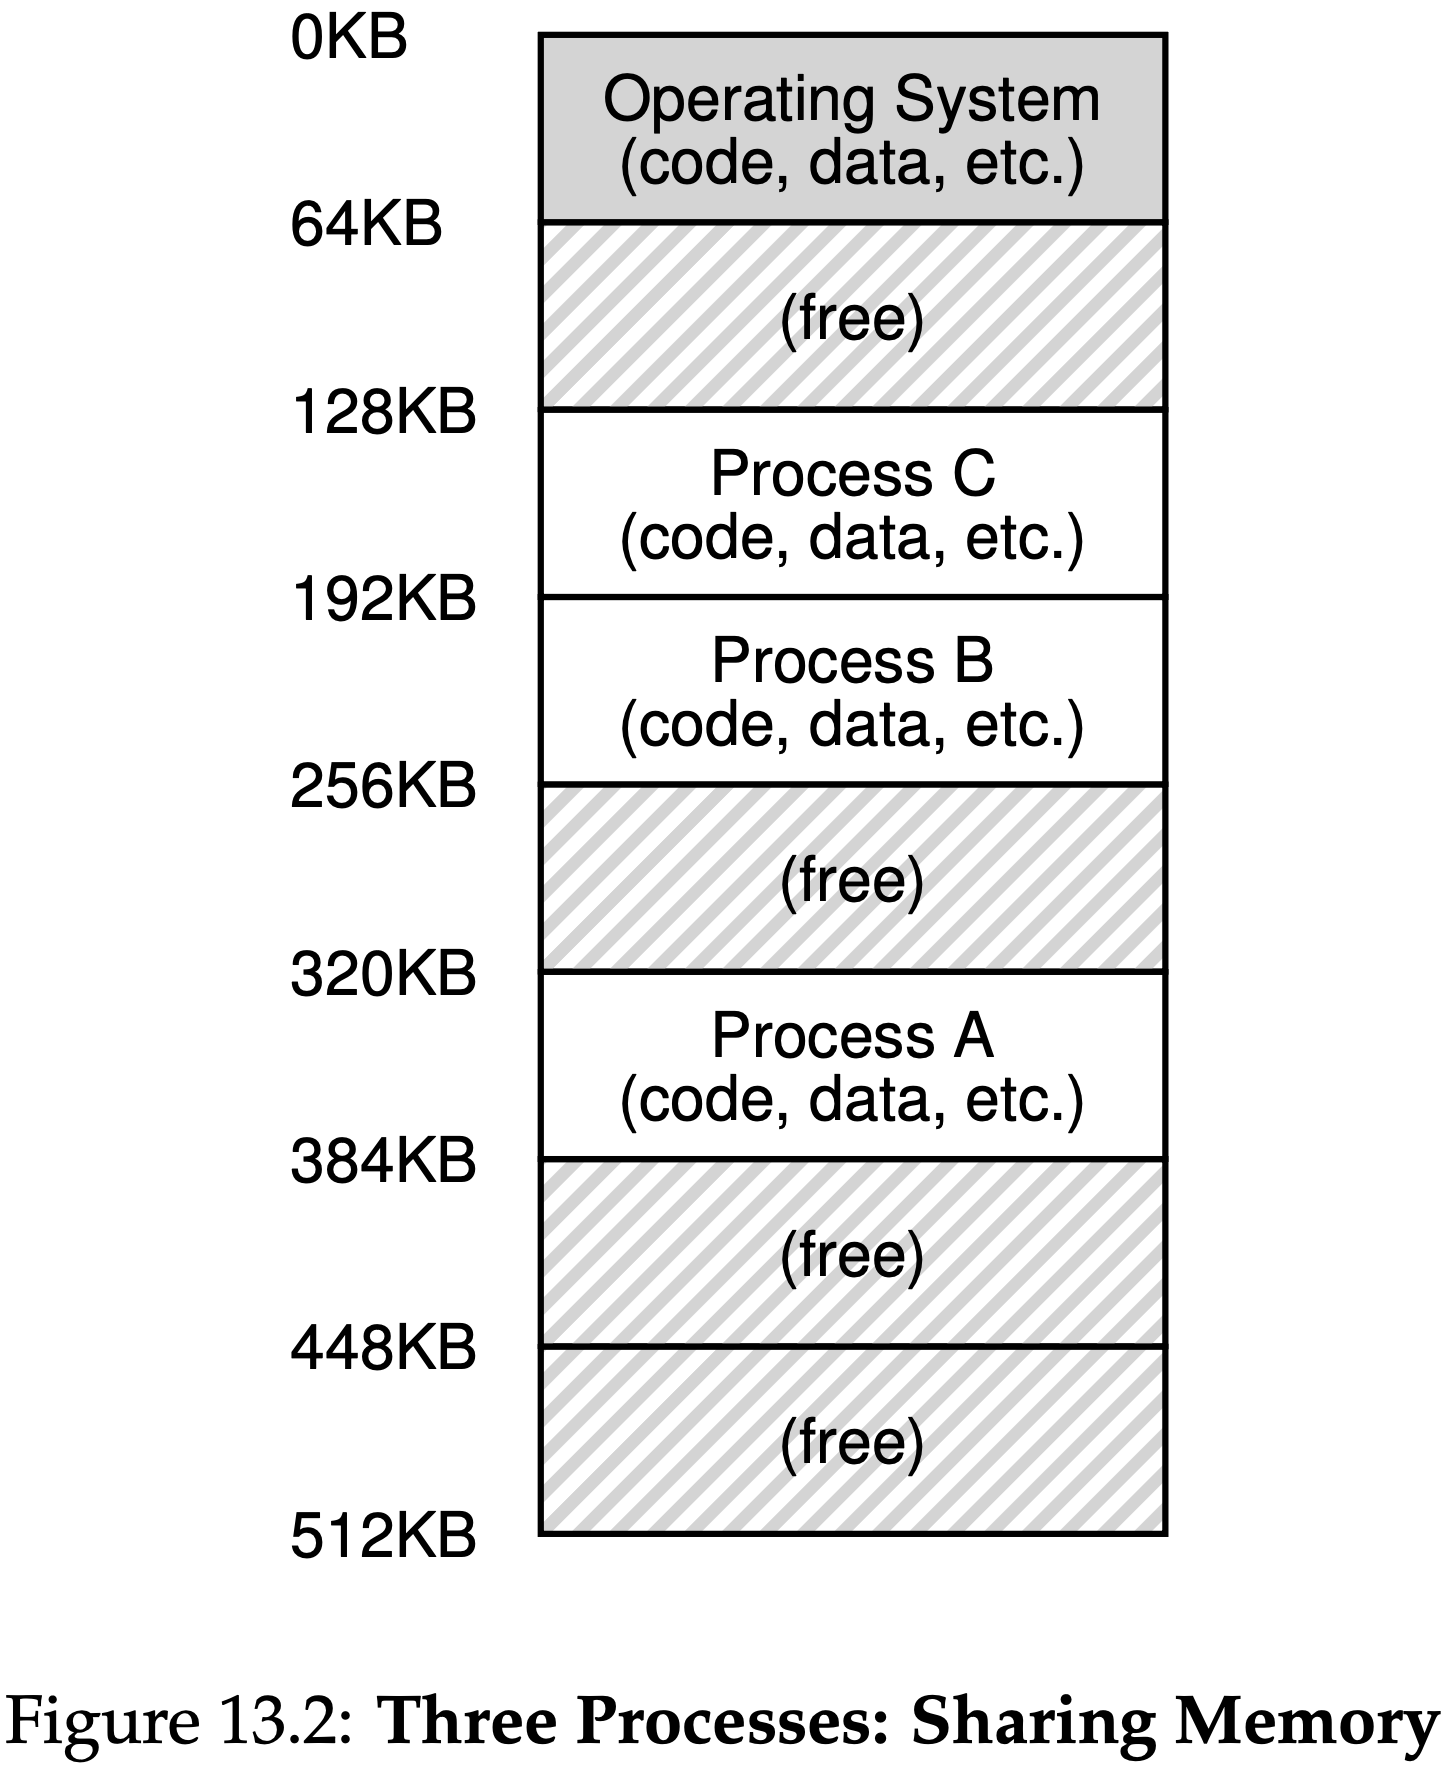
\includegraphics[width=01.1\linewidth]{figs/chapter-13/figure-13.2.png}
            \caption*{Source: chapter page 3.}
            \label{fig:figure-13.2}
        \end{figure}

        \end{column}
    \end{columns}
\end{frame}


\begin{frame}{The Address Space}
    \begin{block}{Address Space}
        The running program's view of memory in the system.
    \end{block}

    \begin{itemize}
        \item The address space contains all memory state of a program.
        \item Main components:
        \begin{itemize}
            \item \textbf{Code}: program instructions;
            \item \textbf{Stack}: function calls, local variables,
                  parameters, and return values;
            \item \textbf{Heap}: dynamically allocated,
                  user-managed memory.
        \end{itemize}
    \end{itemize}
\end{frame}


\begin{frame}{An Example Address Space}
    \begin{columns}
        \begin{column}{0.47\textwidth}
            \begin{itemize}
                \item Example: a small 16KB address space.
                \item Code is static and occupies a fixed region.
                \item Heap and stack can grow and shrink.
                \item They are placed at opposite ends to allow
                      both regions to grow.
                \item This particular organization is a convention,
                      not a requirement.
            \end{itemize}
        \end{column}

        \begin{column}{0.50\textwidth}

        \begin{figure}
            \centering
            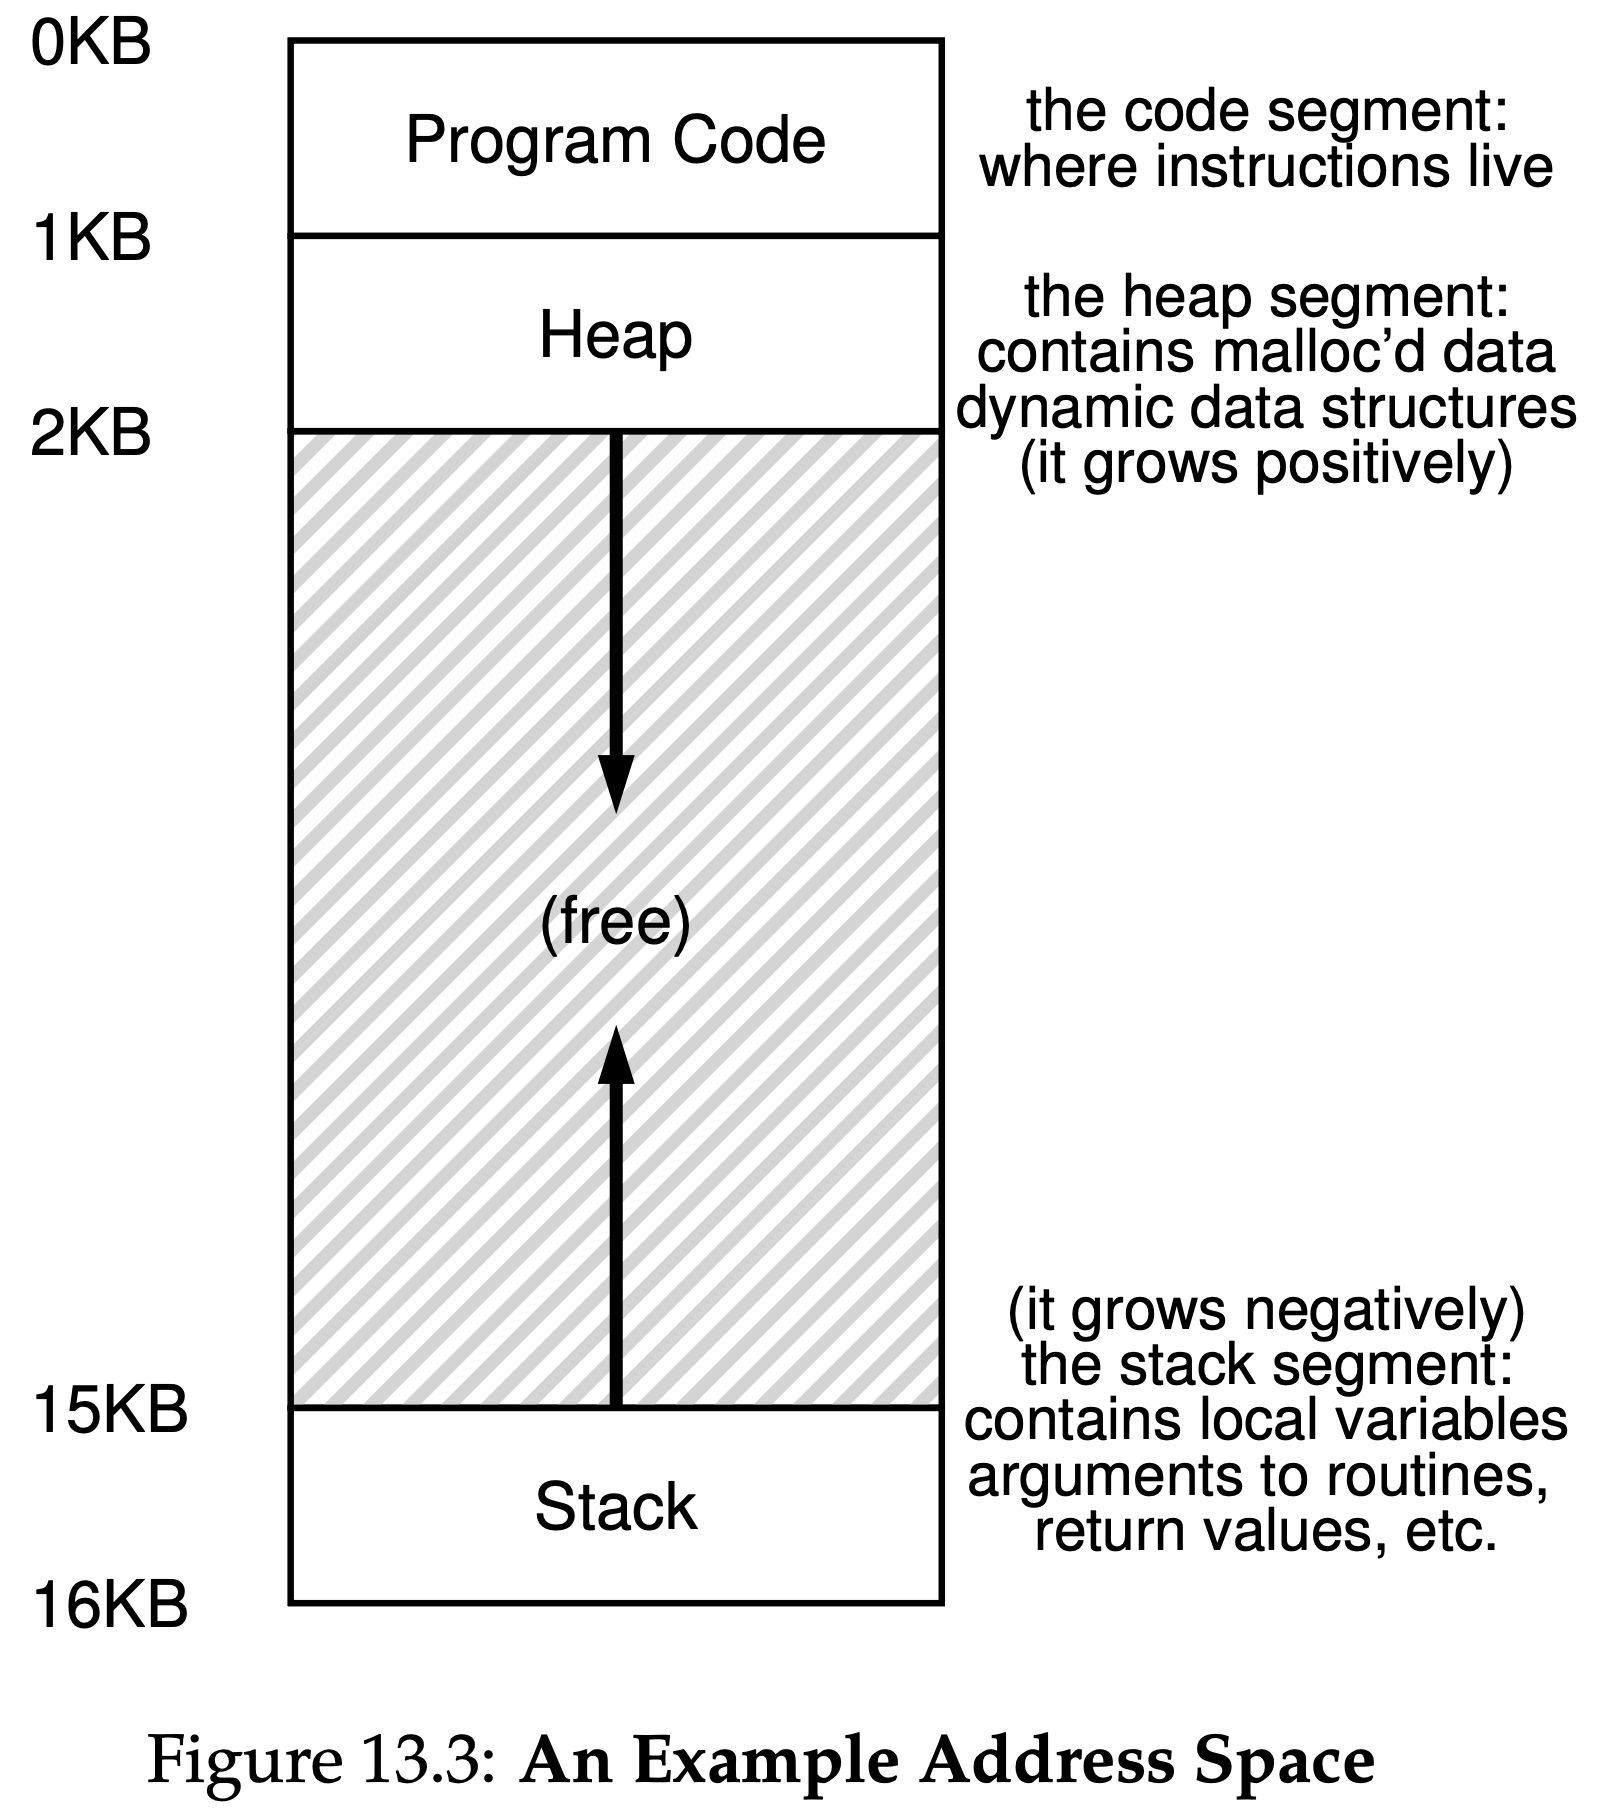
\includegraphics[width=1.1\linewidth]{figs/chapter-13/figure-13.3.png}
            \caption*{Source: chapter page 4.}
            \label{fig:figure-13.3}
        \end{figure}

        \end{column}
    \end{columns}
\end{frame}


\begin{frame}{Address Space: Abstraction vs.\ Reality}
    \begin{itemize}
        \item The address space is an \textbf{abstraction} provided
              by the OS.
        \item A program may behave as if it occupies addresses
              starting at address 0.
        \item In reality, it can reside at arbitrary locations in
              physical memory.
        \item Thus, the address observed by a program is not necessarily
              the physical address used to access memory.
    \end{itemize}

    \begin{center}
        \small
        Compare the virtual view in Figure 13.3 with the physical
        placement of processes in Figure 13.2.
    \end{center}
\end{frame}


\begin{frame}{The Crux: How to Virtualize Memory}
    \begin{block}{The Crux}
        How can the OS build the abstraction of a private,
        potentially large address space for multiple running processes,
        all sharing a single physical memory?
    \end{block}

    \begin{itemize}
        \item The OS is \textbf{virtualizing memory}.
        \item Programs generate \textbf{virtual addresses}.
        \item The OS, together with hardware support, maps them to
              the appropriate \textbf{physical addresses}.
        \item Example: process A's virtual address 0 may correspond
              to physical address 320KB.
    \end{itemize}

    % Figure reference:
    % Figure 13.2 illustrates Process A beginning at physical address 320KB.
\end{frame}


\begin{frame}{Goals of Virtual Memory}
    \begin{description}
        \item[Transparency]
        Virtualization should be invisible to the running program.

        \item[Efficiency]
        Virtualization should be efficient in both time and space;
        hardware support such as TLBs is important.

        \item[Protection]
        Processes must be protected from one another, and the OS
        must be protected from processes.
    \end{description}
\end{frame}


\begin{frame}{Tip: The Principle of Isolation}
    \begin{block}{Isolation}
        If two entities are properly isolated, one can fail without
        affecting the other.
    \end{block}

    \begin{itemize}
        \item Operating systems isolate processes from one another.
        \item Memory isolation prevents programs from affecting
              other processes.
        \item It also prevents programs from affecting the
              underlying OS.
        \item Some systems extend isolation within the OS itself,
              as in \textbf{microkernel} designs.
    \end{itemize}
\end{frame}


\begin{frame}[fragile]{Aside: Every Address You See Is Virtual}
    \begin{itemize}
        \item Any address visible to a user-level program is a
              \textbf{virtual address}.
        \item This includes addresses of code, heap objects, and
              stack variables.
    \end{itemize}

    \begin{columns}
        \begin{column}{0.55\textwidth}
\begin{footnotesize}
\begin{verbatim}
printf("location of code : %p\n", main);
printf("location of heap : %p\n",
       malloc(100e6));

int x = 3;
printf("location of stack: %p\n", &x);
\end{verbatim}
\end{footnotesize}
        \end{column}

        \begin{column}{0.42\textwidth}
            \begin{itemize}
                \item Code appears first.
                \item Heap follows code.
                \item Stack lies near the other end of the
                      virtual address space.
            \end{itemize}
        \end{column}
    \end{columns}

    \begin{alertblock}{Remember}
        Only the OS and hardware know where these values actually
        reside in physical memory.
    \end{alertblock}
\end{frame}


\begin{frame}{Virtual Memory: Summary}
    \begin{itemize}
        \item Virtual memory provides the illusion of a
              \textbf{large, sparse, private address space}.
        \item Each address space contains the program's instructions
              and data.
        \item Programs reference memory through
              \textbf{virtual addresses}.
        \item The OS and hardware translate virtual addresses into
              \textbf{physical addresses}.
        \item The OS provides this abstraction to many processes
              while maintaining \textbf{protection and isolation}.
        \item Virtual memory requires both mechanisms and policies.
    \end{itemize}
\end{frame}